% -*-cap2.tex-*-
% Este fichero es parte de la plantilla LaTeX para
% la realización de Proyectos Final de Carrera, protegido
% bajo los términos de la licencia GFDL.
% Para más información, la licencia completa viene incluida en el
% fichero fdl-1.3.tex

% Copyright (C) 2009 Pablo Recio Quijano 

% MANUAL PARA AÑADIR NUEVOS JUGADORES

\section{Nuevos jugadores}

El diseño de Dominous permite que se puedan añadir nuevos jugadores al sistema de forma sencilla y sin que se requiera
conocimientos de Inteligencia Artificial por parte del usuario, aunque sí se necesitarán ciertas habilidades que se
comentarán a continuación. Podemos crear nuevos usuario \\

Los jugadores de Dominous se guardan dentro del directorio \comando{players}. Cada jugador cuenta con un directorio
donde se almacenan los tres ficheros principales que necesita, que son los siguientes:

\begin{description}
    \item[player.ini] Configuración e información sobre el jugador.
    \item[player.py] Lógica o base de conocimiento del jugador.
    \item[image.png] Avatar o fotografía del jugador, que permite identificarlo y diferenciarlo en el juego.
\end{description}

Para crear un nuevo jugador basta con utilizar estos tres ficheros, colocarlos dentro de su directorio y listo. Automáticamente
el sistema detectará al arrancar que existe un jugador nuevo y lo mostrará disponible en las pantallas de juego y en el
modo laboratorio. \\

A continuación vamos a describir cada uno de los ficheros que se requieren para el correcto funcionamiento de 
nuestro jugador.

\section{Configuración del jugador --- player.ini}

Este fichero de configuración sigue el formato de los ficheros INI --- descrito en el capítulo de implementación --- por
comodidad y rapidez de edición, ya que se puede modificar con cualquier editor de texto plano. El contenido del fichero
debe mostrar los siguientes pares de clave -- valor dentro del grupo \comando{Player}:

\begin{description}
    \item[name] Nombre del jugador. Se utilizará en menús, pantallas, juego o cualquier otro sitio que requiera su uso,
        y también se almacenará en los ficheros de partida.
    \item[image] Avatar o imagen del jugador. Desde aquí podemos definir el nombre del fichero, aunque se recomienda que
        se emplee el nombre por defecto \comando{image.png}. La imagen debe estar en formato PNG, no se requiere transparencia
        y debe tener un tamaño de 150 por 150 píxeles.
    \item[weight] Peso relativo que se utilizará cuando se muestre al jugador dentro de una colección mayor de jugadores.
        Principalmente se usa para la página de selección de jugador, con la idea de que puedan estar ordenados según
        el criterio que se quiera --- en principio, estarán ordenados por nivel de dificultad. El peso debe ser un número
        entero positivo.
\end{description}

Un ejemplo de fichero es el siguiente:

\begin{lstlisting} [language=Python, numbers=left]
[Player]
name = ignacio
image = image.png
weight = 6
\end{lstlisting}

Como vemos, la idea es que el juego sea extensible y, en un futuro, se puedan añadir cómodamente más características
al fichero INI y dotar a los jugadores de más posibilidades.


\section{Base de conocimiento --- player.py}

Para poder desarrollar una base de conocimiento es necesario contar con un mínimo de conocimientos de Python, ya que
la programación del mismo se realiza con este lenguaje de programación. \\

Dos grandes ventajas de Python en este aspecto
es que, por un lado, no es necesario compilar los ficheros \comando{player.py} ya que el lenguaje es interpretado y
el intérprete es el encargado de generar el fichero \comando{player.pyc}, y por otro lado la sencilla sintaxis de Python
lo hacen perfecto para que usuarios sin grandes conocimientos de programación puedan desarrollar un nuevo jugador
de forma sencilla y cómoda, sin miedo a provocar errores lógicos al definir una variable o sintácticos al olvidar
un punto y coma. \\

La forma más cómoda de comenzar a desarrollar un nuevo jugador es partir de uno ya existente --- al igual que sucede
con la creación de nuevos temas gráficos, que veremos en el siguiente apéndice. A la hora de crear un nuevo jugador
controlado por la máquina debemos prestar atención a la función de inicialización de nuestra clase jugador:

\begin{lstlisting} [caption={Inicialización básica de un jugador}, language=Python, numbers=left]
class Player:
    def __init__(self, dealed_tiles):
        self.knowledge = []
        self.knowledge.append([put_any_double()])
        self.knowledge.append([put_anyone()])
\end{lstlisting}

Para mayor legibilidad del ejemplo, eliminamos parte del contenido para destacar el núcleo de nuestro jugador. La base de
conocimiento se define en el atributo \comando{knowledge}, que no es más que una lista del tipo de contenido nativo de Python.
Dentro de esta lista vamos introduciendo las funciones de la biblioteca que queremos que utilice nuestro jugador, de forma
ordenada según la prioridad que queramos que tenga cada función. \\

En el ejemplo, vemos que nuestro jugador, cada vez que tenga que colocar una ficha, intentará, por este orden:
\begin{enumerate}
    \item Colocar una ficha doble, es decir, una ficha cuyos dos lados tengan el mismo número.
    \item Si esto no es posible, intentará colocar una ficha cualquiera.
\end{enumerate}

Como opción por defecto, si ninguna de nuestras reglas se puede ejecutar, el sistema colocará una ficha al azar --- de entre
las posibles candidatas --- o pasará el turno al siguiente jugador. \\

También podemos dotar de cierta aleatoriedad a nuestro sistema. Si en lugar de una lista básica definimos una lista de listas,
se ejecutará aleatoriamente cualquiera de las definidas para un mismo peso. Veamos el siguiente ejemplo:

\begin{lstlisting} [caption={Base de conocimiento avanzada}, language=Python, numbers=left]
class Player:
    def __init__(self, dealed_tiles):
        self.knowledge = []
        self.knowledge.append([
            put_any_double(),
            weight_matrix()
        ])
        self.knowledge.append([put_anyone()])
\end{lstlisting}

En un primer momento se ejecutará, aleatoriamente, una regla entre \textbf{put\_any\_double()} y \textbf{weight\_matrix()}.
Si no hay suerte con la primera, se intentará con la segunda, y si no hay éxito con ninguna se ejecutará el siguiente
conjunto de reglas --- en este caso, \textbf{put\_anyone()}, es decir, intentar colocar una ficha cualquiera.


\section{Imagen o avatar --- image.png}

Como ya hemos comentado antes, esta será la imagen que identifique al jugador, debe estar en formato PNG y debe un tamaño
de 150 por 150 píxeles. Se recomienda que sea una imagen clara y sencilla, y para seguir con la misma línea gráfica debería
ser una fotografía real con un cierto efecto de envejecimiento con un tintado de color naranja.

\begin{figure}[h]
  \begin{center}
    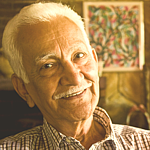
\includegraphics[scale=0.5]{avatar_jugador.png}
  \end{center}
  \caption{Ejemplo de imagen válida como avatar de jugador.}
  \label{fig:avatar_jugador}
\end{figure}

